\documentclass[11pt,a4paper]{article}

\usepackage[landscape,margin=10mm]{geometry}
\usepackage{fontspec}
\usepackage{xcolor}
\usepackage{tikz}
\usetikzlibrary{arrows.meta,positioning,shadows}
\usepackage[most]{tcolorbox}
\usepackage{microtype}

\setmainfont{DejaVu Sans}
\pagestyle{empty}

\definecolor{Brand}{HTML}{155E46}
\definecolor{BrandDark}{HTML}{103F31}
\definecolor{GreenSoft}{HTML}{E8F4EE}
\definecolor{Blue}{HTML}{246B8E}
\definecolor{BlueSoft}{HTML}{E9F3F8}
\definecolor{Orange}{HTML}{B65F24}
\definecolor{OrangeSoft}{HTML}{FFF0E5}
\definecolor{Purple}{HTML}{7156A5}
\definecolor{PurpleSoft}{HTML}{F1ECFA}
\definecolor{Red}{HTML}{A74343}
\definecolor{RedSoft}{HTML}{FBECEC}
\definecolor{Gold}{HTML}{967118}
\definecolor{GoldSoft}{HTML}{FBF5DE}
\definecolor{Ink}{HTML}{18211C}
\definecolor{Muted}{HTML}{66736C}

\begin{document}

\begin{center}
  {\LARGE\bfseries\color{Ink} Research-Mind: Future Scope Mind Map}\par
  \vspace{1mm}
  {\small\color{Muted}Har item mein: \textbf{What → How} --- interviewer ke implementation question ke liye}
\end{center}

\vspace{2mm}

\begin{center}
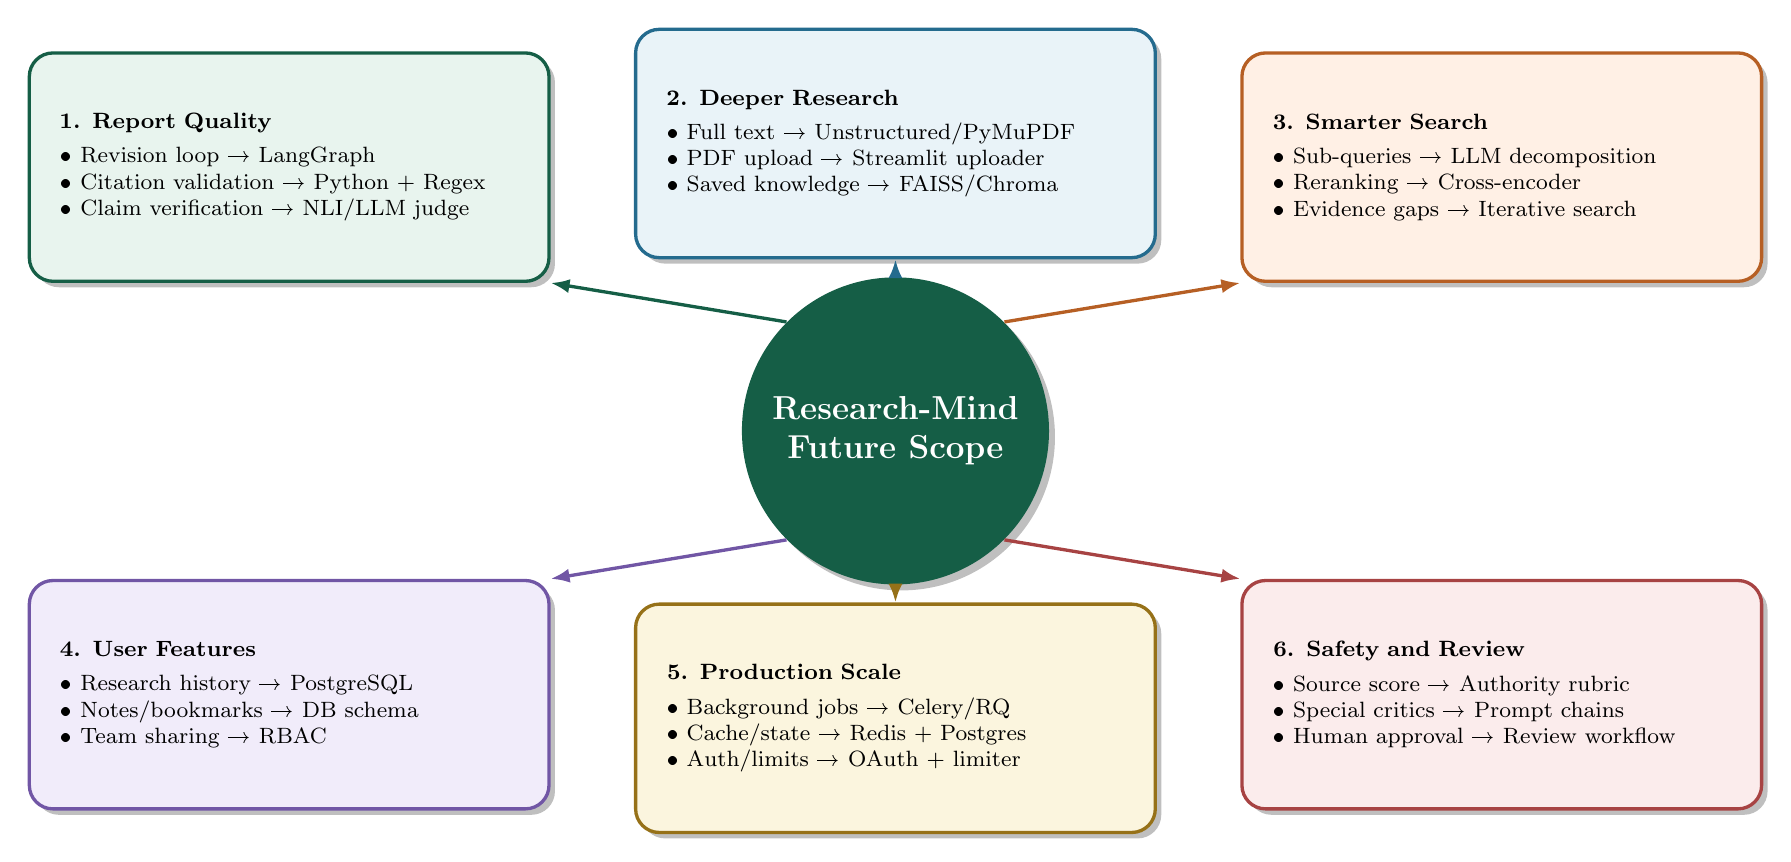
\begin{tikzpicture}[
  line/.style={-{Latex[length=2.4mm]},very thick,rounded corners=3mm},
  center/.style={circle,minimum size=39mm,align=center,fill=Brand,text=white,
                 font=\bfseries\large,drop shadow},
  branch/.style={rounded corners=3mm,minimum height=29mm,text width=58mm,
                 align=left,inner sep=4mm,draw,very thick,drop shadow,
                 font=\footnotesize}
]

  \node[center] (core) at (0,0) {Research-Mind\\Future Scope};

  \node[branch,fill=GreenSoft,draw=Brand] (quality) at (-7.7,3.35) {
    \textbf{1. Report Quality}\\[1mm]
    \textbullet\ Revision loop → LangGraph\\
    \textbullet\ Citation validation → Python + Regex\\
    \textbullet\ Claim verification → NLI/LLM judge
  };

  \node[branch,fill=BlueSoft,draw=Blue] (knowledge) at (0,3.65) {
    \textbf{2. Deeper Research}\\[1mm]
    \textbullet\ Full text → Unstructured/PyMuPDF\\
    \textbullet\ PDF upload → Streamlit uploader\\
    \textbullet\ Saved knowledge → FAISS/Chroma
  };

  \node[branch,fill=OrangeSoft,draw=Orange] (search) at (7.7,3.35) {
    \textbf{3. Smarter Search}\\[1mm]
    \textbullet\ Sub-queries → LLM decomposition\\
    \textbullet\ Reranking → Cross-encoder\\
    \textbullet\ Evidence gaps → Iterative search
  };

  \node[branch,fill=PurpleSoft,draw=Purple] (product) at (-7.7,-3.35) {
    \textbf{4. User Features}\\[1mm]
    \textbullet\ Research history → PostgreSQL\\
    \textbullet\ Notes/bookmarks → DB schema\\
    \textbullet\ Team sharing → RBAC
  };

  \node[branch,fill=GoldSoft,draw=Gold] (scale) at (0,-3.65) {
    \textbf{5. Production Scale}\\[1mm]
    \textbullet\ Background jobs → Celery/RQ\\
    \textbullet\ Cache/state → Redis + Postgres\\
    \textbullet\ Auth/limits → OAuth + limiter
  };

  \node[branch,fill=RedSoft,draw=Red] (safety) at (7.7,-3.35) {
    \textbf{6. Safety and Review}\\[1mm]
    \textbullet\ Source score → Authority rubric\\
    \textbullet\ Special critics → Prompt chains\\
    \textbullet\ Human approval → Review workflow
  };

  \draw[line,color=Brand] (core.north west) -- (quality.south east);
  \draw[line,color=Blue] (core.north) -- (knowledge.south);
  \draw[line,color=Orange] (core.north east) -- (search.south west);
  \draw[line,color=Purple] (core.south west) -- (product.north east);
  \draw[line,color=Gold] (core.south) -- (scale.north);
  \draw[line,color=Red] (core.south east) -- (safety.north west);

\end{tikzpicture}
\end{center}

\vfill

\begin{tcolorbox}[
  colback=white,colframe=Brand,boxrule=.7pt,arc=2mm,
  left=3mm,right=3mm,top=2mm,bottom=2mm
]
\centering
\textbf{Recommended priority:}
\color{BrandDark}
Citation validation → Writer--Critic revision →
Claim verification → PDF/full-text support → User history → Scale
\end{tcolorbox}

\end{document}
